\newpage
% I leave this here as the example of how to use the pdf call function and not have the title of the section on a different page to the image of the pdf.

 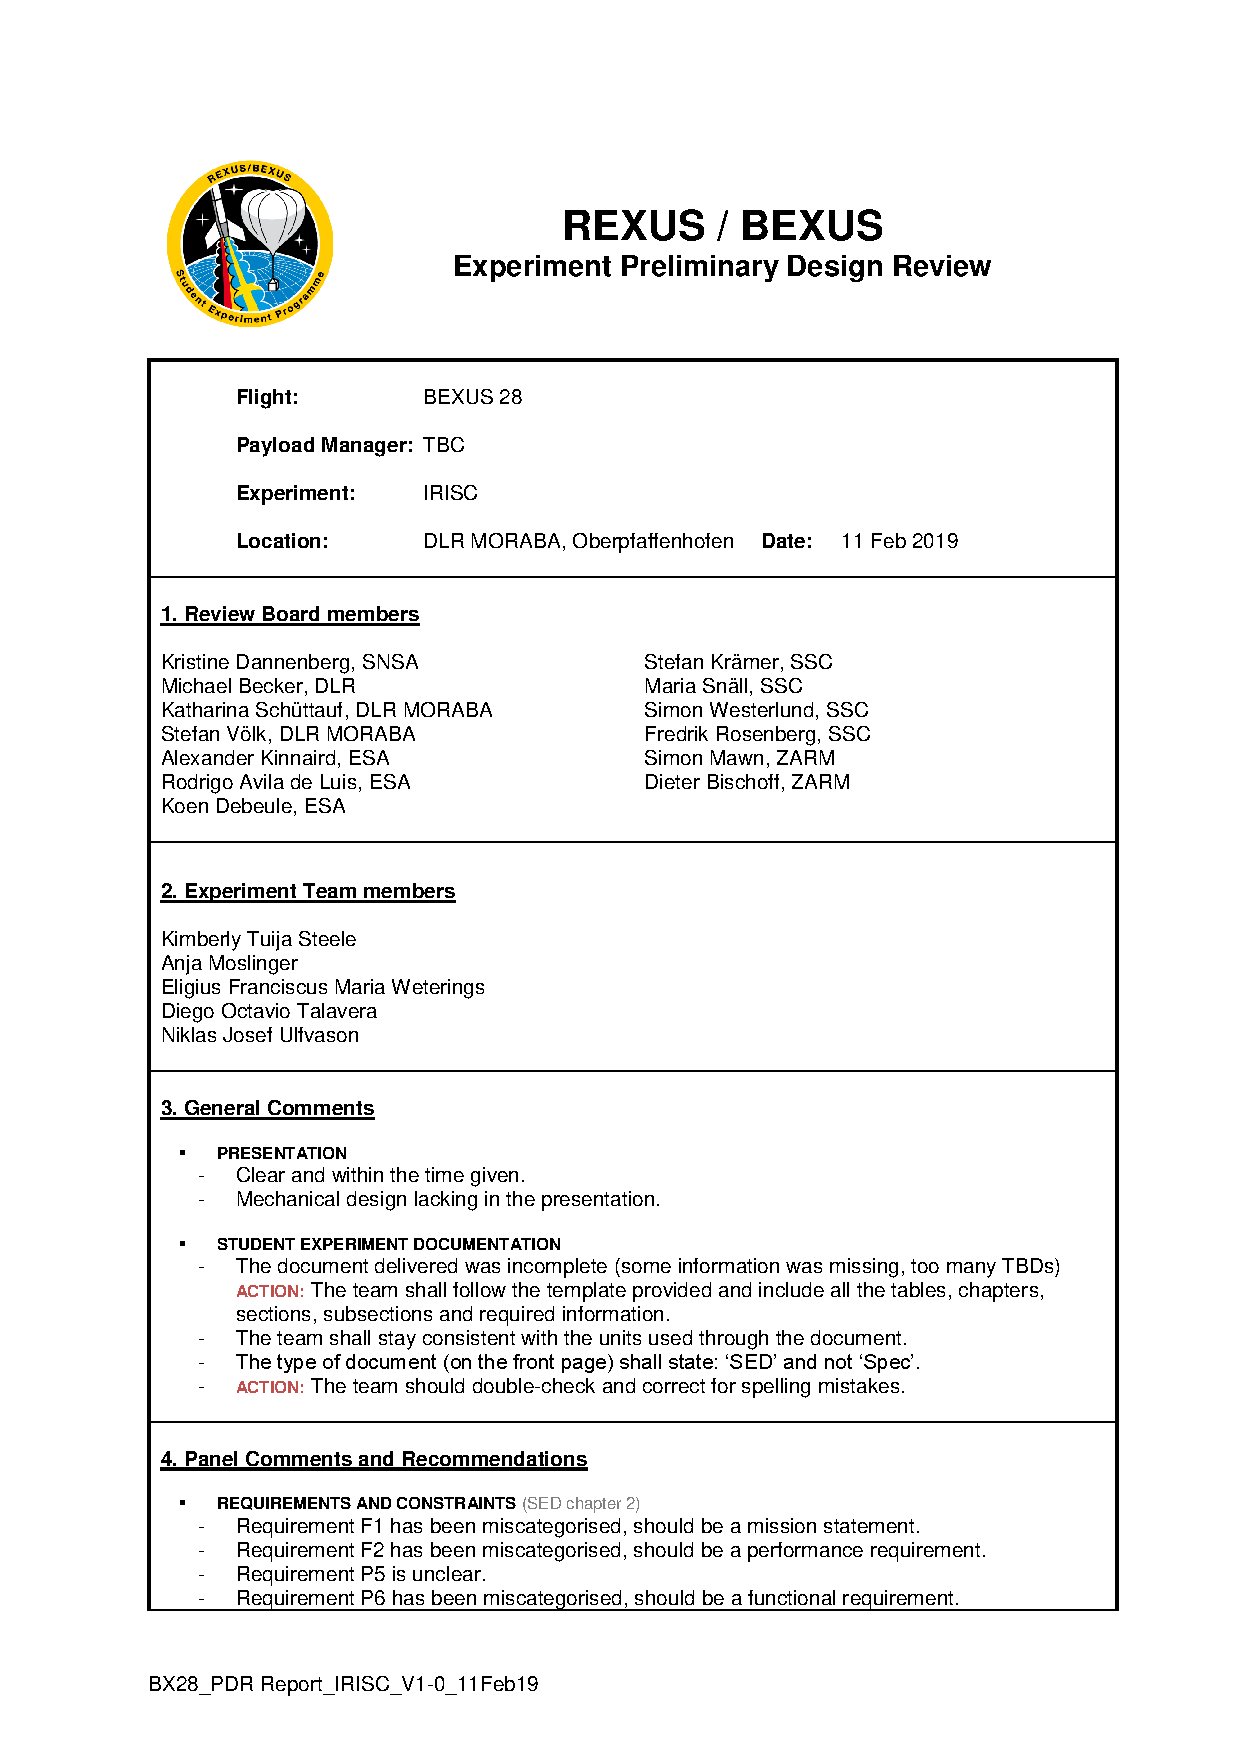
\includepdf[scale=0.8,pages={1},pagecommand=\section{Experiment Reviews}\subsection{Preliminary Design Review (PDR)},offset=0 -1cm]{appendix/ExperimentReviews/PDRReport.pdf}
 \includepdf[scale=0.8,pages={2,3,4},pagecommand={}]{appendix/ExperimentReviews/PDRReport.pdf}
 
 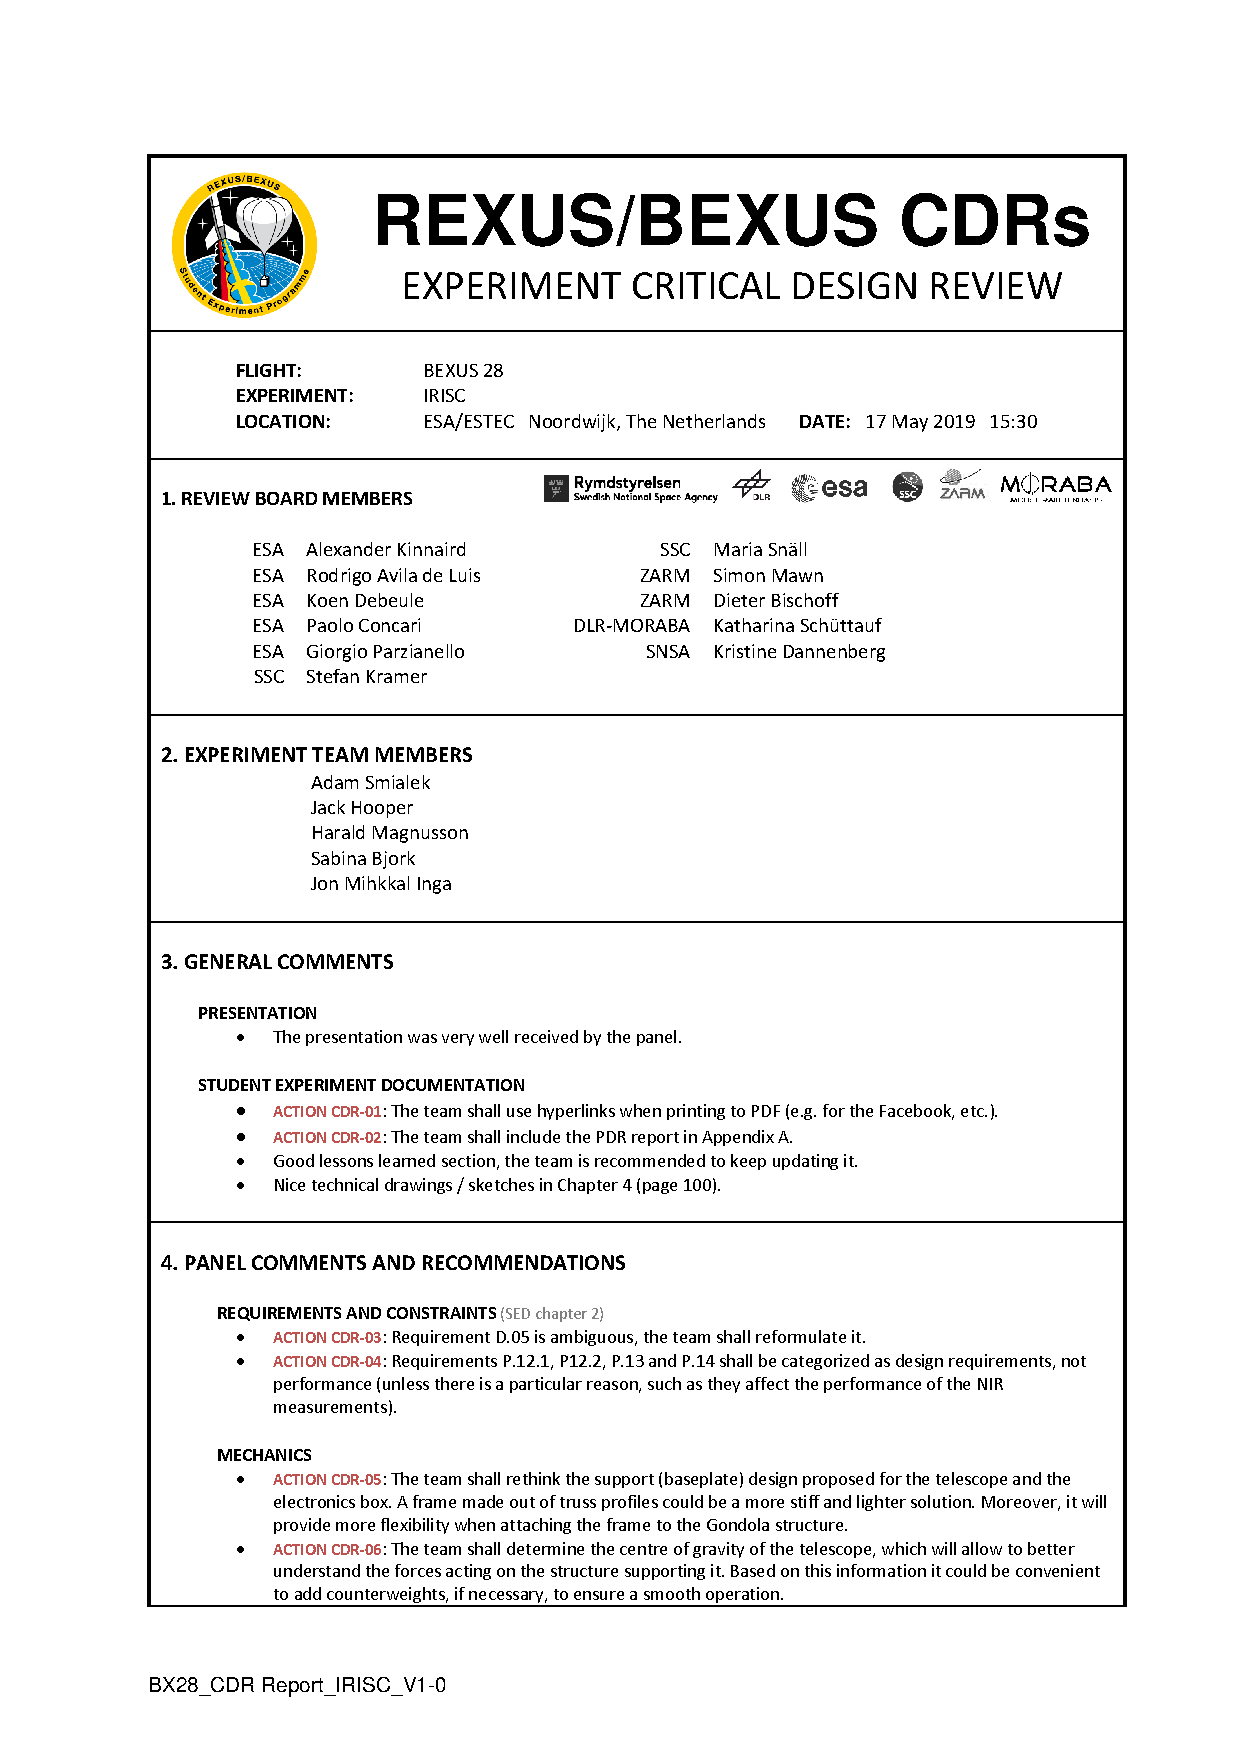
\includepdf[scale=0.8,pages={1}, pagecommand=\subsection{Critical Design Review (CDR)},offset=0 -1cm]{appendix/ExperimentReviews/CDRReport.pdf}
 \includepdf[scale=0.8,pages={2,3,4},pagecommand={}]{appendix/ExperimentReviews/CDRReport.pdf}
 
 
% \includepdf[scale=0.8,pages={1}, pagecommand=\subsection{Integration Progress Review (IPR)},offset=0 -1cm]{appendix/pdf/BX26-IPR-TUBULAR-Report-v1-1-26Jul18.pdf}
% \includepdf[scale=0.8,pages={2,3,4,5,6,7,8},pagecommand={}]{appendix/pdf/BX26-IPR-TUBULAR-Report-v1-1-26Jul18.pdf}

